% !TEX root = main.tex
%%%%%%%%%%%%%%%%%%%%%%%%%%%%%%%%%%%%%%%%%%%%%%%%%%%%%%%%%%%%%%%%%%%%%%%%%%%%%%%%
% Introduction
%%%%%%%%%%%%%%%%%%%%%%%%%%%%%%%%%%%%%%%%%%%%%%%%%%%%%%%%%%%%%%%%%%%%%%%%%%%%%%%%
\section{Introduction}
\label{section:introduction}

The Cray XK7 Titan supercomputer was the \#1 system in the world for a
very long time, and has remained a critically important computer
system through the end of its life in the Summer of 2019. It defied
scale with 18,688 individual compute nodes and delivered tens of
billions of computing hours to the U.S. Oepartment of Energy
mission-critical programs for nearly 7 years.
 
Titan was quite an interesting machine from a reliability perspective.
Its operation was forced to execute three very significant rework cycles, two on
the mechanical assembly affecting the PCIe connector from the GPU
daughtercard to the motherboard, and a replacement of about 11,000 GPU
assemblies because of a failing resistor on a printed circuit board.

Figure~\ref{fig:chronology} illustrates the chronology of the rework
cycles. It shows the number of GPU changes at periodic inventories.
\begin{figure*}[tbp]
  \centering
  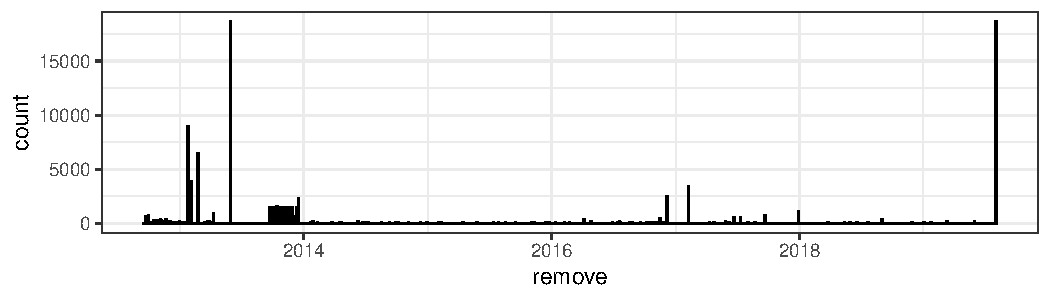
\includegraphics[width=\textwidth]{figs/chronology001.pdf}
  \caption{Daily volume of GPU swaps with labels on most frequent dates.}
  \label{fig:chronology}
\end{figure*}
 
We have conducted a good bit of statistical analysis on the failure
rates of these GPU assemblies, but I want to propose a different topic
that I have not seen for other/similar systems.  I want to complete
the statistical analysis of the failure rates as we near end of life,
looking for the opposite side of the “bathtub curve”.  There is
specific decay associated with the electronic components where, as
these products age, they will eventually fail thresholds for guard
band margin and other things. In a lot of cases, they will just fail
as well. 
 
This machine is quite large, was very important to many people, and I
think this analysis could be very intriguing. 
 
I am looking for help, very specifically with the statistics portion
of this, i.e. what do the failure rates for specific components look
like? What distributions do those failure rates follow? How could
appropriate models extrapolate failure rates beyond the end of service
date (the dotted lines) ? 
 
I have submitted an abstract to a Cray-focused user group and workshop
on this topic, and it has been accepted.  I would like to execute this
statistical analysis and generate a short presentation (30 minutes)
and a short paper (4-8 pages is a likely target).  Presentation is
targeted for May 7-9 (TBD). An initial/working version of the paper
would be due earlier. If we miss that target (April 12), no big
deal. We can finish on a similar schedule as the presentation.  I have
all of the raw data for the component failures, and need the
statistical help to complete the analysis. 
 
Because there is a huge swing in the failure rates of the GPUS from
2016/17 when the resistor problem escalated rapidly out of control, it
is statistically interesting, where we inject fresh material in to an
existing machine. We’d likely want to categorically separate new GPU
assemblies from old and could track the early life failures from those
new 11,000 parts versus the continued failure of the remaining 6000. 
 
George, Christian-  any interest in this? Barney gave it a thumbs
up. I think this is a timely and very interesting topic. 

\fix{Need a description of Titan GPU events timeline. Jim or Don?}
